%Commandi utili ridefiniti

\newcommand{\COURSE}{Programmazione concorrente e distribuita}

\newcommand{\STUDENT}{Grigoras Valentin}
\newcommand{\MATRICOLA}{1099561}
\newcommand{\ANNO}{A.A 2018/2019}




% ----------------------- TODO ---------------------------

\documentclass[a4paper]{scrartcl}
\usepackage[T1]{fontenc}
\usepackage[utf8]{inputenc}
\usepackage[italian]{babel}

\usepackage{fancyhdr}
\usepackage{color}

\usepackage{lastpage}
\usepackage{listings}
\usepackage{tikz}

\usepackage{subfigure}
\usepackage{float}
\usepackage{hyperref}
\usepackage{tabularx}
\usepackage{color}
\usepackage{geometry}
\usepackage{fancybox}

\usepackage{utopia}
\usepackage{lipsum}
\usepackage{amstext}
\usepackage{xcolor}
\usepackage{listingsutf8}
\lstset{inputencoding=utf8/latin1}
\definecolor{blue}{HTML}{007af7}
\definecolor{red}{HTML}{920022}
\definecolor{grey}{HTML}{fdfcf8}
\definecolor{comment}{HTML}{1b9852}
\definecolor{strings}{HTML}{5f283e}

\definecolor{tipo}{RGB}{167, 63, 74}
\definecolor{variabile}{RGB}{32, 114, 154}

\lstset{language=Java,backgroundcolor=\color{grey}, commentstyle=\color{comment},identifierstyle  = \color{blue},extendedchars=true, frame=single,keepspaces=true, keywordstyle=\color{red},tabsize=3,showstringspaces=false,literate={é}{{\'{e}}}1, literate={è}{{\'{e}}}1 }


\input kvmacros

%Größe der Ränder setzen
\geometry{a4paper,left=3cm, right=3cm, top=3cm, bottom=3cm}

%Kopf- und Fußzeile
\pagestyle {fancy}
\fancyhead[L]{\COURSE}
\fancyhead[C]{}
\fancyhead[R]{\rightmark }

\fancyfoot[L]{}
\fancyfoot[C]{}
\fancyfoot[R]{Pagina \thepage /\pageref*{LastPage}}

%Formatierung der Überschrift, hier nichts ändern
\def\header#1#2#3#4{
\vspace*{\fill}
  \begin{center}
    { \Large Appunti di Programmazione Concorrente e Distribuita #1}\\ \vspace{10pt}
    {(\ANNO #2)} \\  \vspace{10pt}
{\Large \STUDENT#3} \\  \vspace{10pt}
{\Large Matricola: \MATRICOLA #4} \\  \vspace{10pt}
  \end{center}
  \vspace*{\fill}
}


\begin{document}

\header{}{}{}{}

\pagebreak

	\renewcommand{\contentsname}{Contenuti}
	\renewcommand\tablename{new}
	\tableofcontents \pagebreak
	\listoffigures \pagebreak

\vspace{30pt}
\section{Metodo \textit{Equals()}}
L’operatore binario == viene utilizzato per stabilire se il contenuto di due variabili è identico. Per i tipi non primitivi viene confrontato il contenuto dei puntatori degli oggetti, ovvero l’indirizzo di memoria degli oggetti a cui i puntatori fanno riferimento.
Spesso però potremmo avere oggetti che nonostante puntino ad indirizzi di memoria differenti possono essere considerati a tutti gli effetti uguali.
La procedura standard per confrontare oggetti in Java è il metodo\textbf{equals()}, definito in \textbf{Object}, quindi è disponibile su tutti gli oggetti (ma non sui tipi primitivi):
\begin{lstlisting}
/*segnatura*/
public boolean equals(Object x)

/*implementazione*/
public boolean equals(Object obj) {
  return this == obj;
}

\end{lstlisting}
Il confronto viene fatto con l’operatore ==, dato che non è possibile conoscere in Object come confrontare qualsiasi oggetto Java.  Per effettuare un confronto migliore non basato sugli indirizzi di memoria, è buona norma effettuare l’overriding del metodo equals in ogni classe che sviluppiamo.

\subsection{Proprietà del metodo \textit{Equals()}}
Il linguaggio Java richiede che qualunque ridefinizione del metodo equals() rispetti determinate proprietà che forniscono una vera e propria \textbf{relazione di equivalenza}:
\begin{itemize}
\item \textbf{Riflessività}; per ogni oggetto x, avremo che x.equals(x) ritorna \textit{true};
\item \textbf{Simmetria}: dati due oggetti x ed y, avremo che se x.equals(y) ritorna true, allora y.equals(x) ritorna \textit{true};
\item \textbf{Transitività}: dati tre oggetti x, y e z, se x.equals(y) ritorna true e y.equals(z) ritorna true, allora x.equals(z) ritorna \textit{true}.
\end{itemize}

\subsection{Corretta implementazione di \textit{Equals()}}
Si devono eseguire 3 step nella classe più un quarto di verifica all'esterno:
\begin{enumerate}
\item Usare == per vedere se l'argomento è uguale a this;
\begin{lstlisting}
if(this == obj) return true;
\end{lstlisting}

\item Verificare se l’oggetto passato al metodo è del tipo desiderato, effettuando un controllo con l’operatore \textit{instanceof}, in caso negativo restituiremo false;
\begin{lstlisting}
if(!(obj istanceof ClassName)) return false;
\end{lstlisting}

\item Essendo sicuri di avere un oggetto del tipo desiderato, potremo effettuare in sicurezza un downcast al tipo desiderato. In questo modo possiamo accedere ai campi e metodi prima nascosti a causa del riferimento di tipo Object utilizzato;
\begin{lstlisting}
NomeClasse cp = (NomeClasse)ogj;
return cp.campo1.equals(this.campo1) &&
 cp.campoN.equals(this.campoN);
\end{lstlisting}

\item Confrontare se stiamo rispettando la riflessibilità, simmetria e transitività.
\end{enumerate}

\begin{figure}[H]
\centering
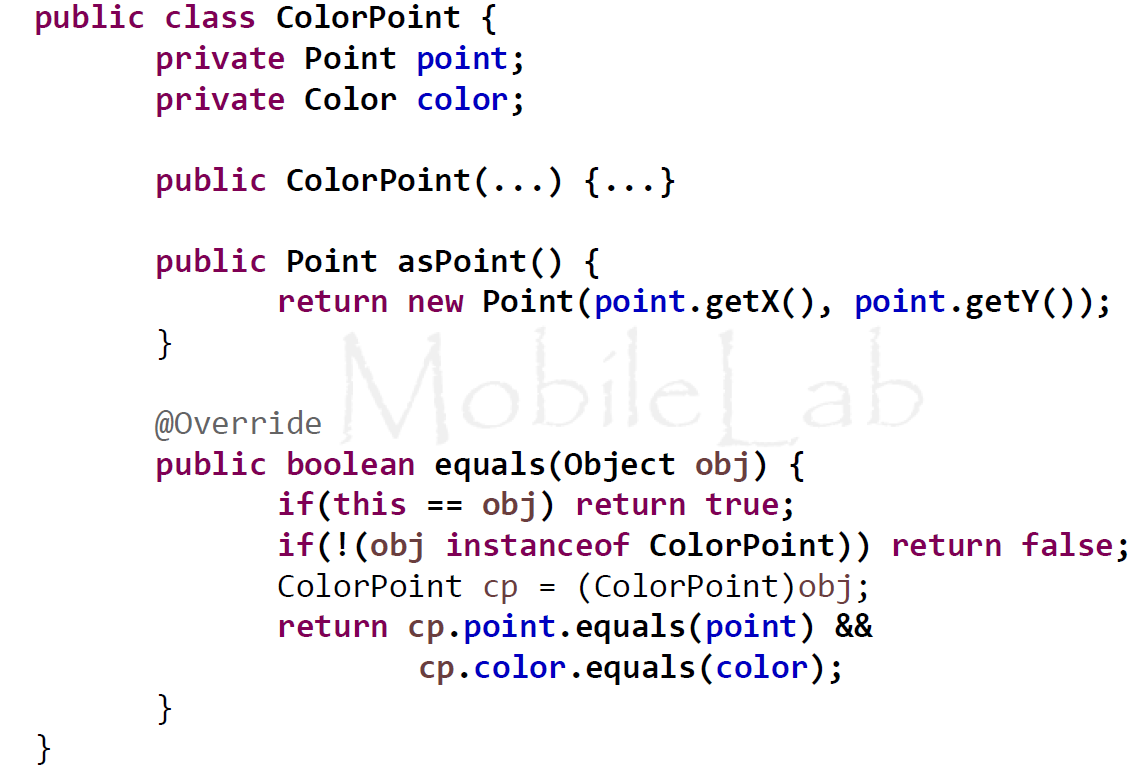
\includegraphics[scale=0.42]{images/imgEquals}
\caption{Implementazione corretta di equals\label{fig:UC3}}
\end{figure}

\subsection{Binding dinamico di \textit{Equals()}}
Quando si effettua l’overriding di equals, è sconsigliato cambiare il tipo del parametro di equals Object , altrimenti non avremo un overriding ma un overloading. Questo cambiamento potrebbe provocare disastri, vediamo con un esempio in cui cambiando il tipo del parametro di equals cosa potrebbe accadere:
\begin{lstlisting}
public boolean equals(Employee e){}
\end{lstlisting}
Inoltre supponeremo di avere:
\begin{lstlisting}
	Emplyee e1 = new Employee(...);
  	Emplyee e2 = new Employee(...);
  	Object o1 = e1;
  	Object o2= e1;
\end{lstlisting}
 Analizziamo cosa succede ad ogni riga con l’utilizzo del Binding dinamico:
\begin{itemize}
\item \textbf{o1.equals(o2);} Le firme candidate sono cercate solo in Object perché il tipo dichiarato di o1 è Object. Di conseguenza non verrà considerata la specializzazione del metodo equals effettuata;
\item \textbf{o1.equals(e2);} Nella fase 2 del Binding dinamico non c’è overriding , quindi verrà preso l’unico metodo equals esattamente uguale che sarà quello contenuto in Object. Anche in questo caso non verrà considerata la specializzazione del metodo equals che abbiamo effettuato;
\item \textbf{e1.equals(o1);} Viene valutato ma Object non è assegnabile a Employee. Di conseguenza non verrà considerata la specializzazione del metodo equals effettuata;
\item \textbf{e1.equals(e2);} La firma combacia con quella specializzata e sarà l’unico caso in cui verrà chiamato il “giusto” equals.
\end{itemize}

\subsection{Metodo \textit{Equals()} ed eredità}
Quando il metodo equals viene sovrascritto bisogna prestare attenzione al funzionamento tra il metodo equals definito e il suo funzionamento nelle classi sottostanti. In definitiva bisogna decidere come si deve comportare il metodo equals con le sue sottoclassi. In particolare, bisogna porsi due domande:

\begin{enumerate}
\item \textbf{Il criterio di confronto tra oggetti di una sottoclasse è diverso da quello che vale tra oggetti della superclasse?}
\begin{itemize}
\item No, allora bisogna definire equals della superclasse final in modo che nessuna sottoclasse possa sovrascriverlo;
\item Si, allora il metodo equals deve essere opportunamente ridefinito in ogni sottoclasse in cui il criterio di confronto è differente.
\end{itemize}
\item \textbf{Un oggetto di una sottoclasse può essere considerato uguale ad un oggetto di una superclasse?}
\begin{itemize}
\item No, allora bisogna verificare di ammettere il confronto solo tra agli oggetti del tipo giusto;
\item Si, allora se gli oggetti di una sottoclasse possono essere considerati uguali a quelli di una superclasse dovremo ammettere al confronto tutti gli oggetti di quel tipo e tutte le sue sottoclassi.
\end{itemize}
\end{enumerate}

\subsection{Tipi primitivi vs oggetti}
Si sente dire spesso l’affermazione \textit{in Java tutto è un oggetto}. In realtà questa frase non è del tutto vera in quanto esistono i tipi primitivi che permettono di utilizzare numeri, caratteri e valori booleani senza ricorrere agli oggetti. I tipi primitivi sono riconoscibili anche perché iniziano con una lettera minuscola (mentre i nomi delle classi iniziano sempre con una maiuscola). I tipi primitivi disponibili in Java sono i seguenti:
\begin{itemize}
\item \textbf{boolean:} valore booleano, può assumere i valori true e false;
\item \textbf{byte:} numero intero a 8 bit;
\item \textbf{short:} numero intero a 16 bit;
\item \textbf{int:} numero intero a 32 bit;
\item \textbf{long:} numero intero a 64 bit;
\item \textbf{float:} numero reale a 32 bit in virgola mobile (IEEE 754-1985);
\item \textbf{double:} numero reale a 64 bit in virgola mobile (IEEE 754-1985);
\item \textbf{char:} carattere unicode a 16 bit;
\end{itemize}
Gli oggetti in Java sono istanze di una classe.
Una delle differenze importanti fra tipi primitivi e oggetti si ha se guardiamo la situazione della memoria a basso livello. Infatti nella locazione di memoria corrispondente a un tipo primitivo è presente il valore mentre in quella di un oggetto è presente il puntatore all’area di memoria che contiene l’oggetto. Un diagramma spiega meglio questa differenza:
\begin{lstlisting}
int i1 = 5;
int i2 = 7;
Persona p1 = new Persona("Mario", "Rossi");
Persona p2 = new Persona("Mario", "Verdi");
\end{lstlisting}
\begin{figure}[H]
\centering
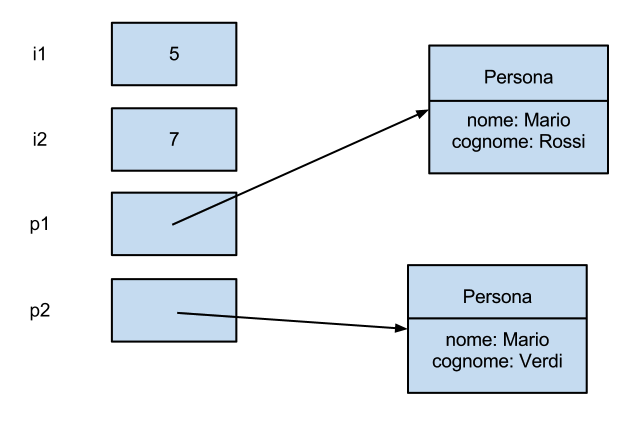
\includegraphics[scale=0.42]{images/tipiPrimitivi}
\caption{tipi primitivi e oggetti: rappresentazione in memoria\label{fig:UC3}}
\end{figure}
Fin qui sembra tutto semplice, andiamo avanti facendo un po’ di assegnazioni:
\begin{lstlisting}
i2 = i1;
p2 = p1;
\end{lstlisting}
A questo punto quale è la situazione? Ovviamente i1 e i2 assumo lo stesso valore, stessa cosa anche per p1 e p2. Ma se andiamo a vedere cosa è successo in memoria la situazione è un po’ più complicata: 	
\begin{figure}[H]
\centering
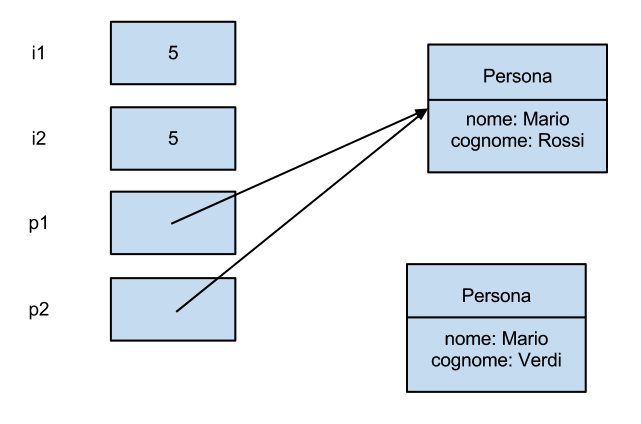
\includegraphics[scale=0.42]{images/memoria1}
\caption{tipi primitivi e oggetti: rappresentazione in memoria dopo assegnazione\label{fig:UC3}}
\end{figure}
Adesso p1 e p2 puntano allo stesso oggetto: abbiamo una condivisione di memoria che può risultare pericolosa se non gestita adeguatamente. Infatti richiamando un metodo setter su uno dei due oggetti (per esempio p1.setNome("Fabio")) si modificherà l’oggetto condiviso dai due puntatori. 

\subsection{\textit{Equals()} Vs ==}
Iniziamo con l’operatore ==: invocando questo costrutto viene confrontato il valore contenuto nella variabile. Quindi, nel caso di tipi primitivi viene confrontato il valore vero, mentre nel caso di oggetti viene confrontato l’indirizzo di memoria a cui i puntatori fanno riferimento.
Vediamo un esempio concreto. Il seguente codice stampa sulla console 4 volte il valore true:
\begin{lstlisting}
int i1 = 5;
int i2 = 7;
 
System.out.println(i1 != i2);
i2 = i1;
System.out.println(i1 == i2);
 
Persona p1 = new Persona("Mario", "Rossi");
Persona p2 = new Persona("Mario", "Verdi");
 
System.out.println(p1 != p2);
p2 = p1;
System.out.println(p1 == p2);
\end{lstlisting}
p1 e p2 puntano allo stesso oggetto e quindi confrontando l’indirizzo di memoria corrispondente al puntatore si ha un esito positivo.
Vediamo un altro esempio leggermente più complicato. Definiamo due volte lo stesso valore/oggetto e confrontiamolo con ==:
\begin{lstlisting}
int i1 = 5;
int i2 = 5;
 
System.out.println(i1 == i2);
 
Persona p1 = new Persona("Mario", "Rossi");
Persona p2 = new Persona("Mario", "Rossi");
 
System.out.println(p1 == p2);
\end{lstlisting}
In questo caso la prima condizione sui tipi primitivi è vera mentre quella sugli oggetti è falsa! Il motivo è chiaro, le variabili p1 e p2 in questo caso puntano a locazioni di memoria diverse quindi confrontando gli indirizzi di memoria si avrà un risultato negativo. Per ovviare a questo problema è necessario usare il metodo equals che, a differenza dell’operatore ==, confronta gli oggetti puntati entrando quindi in merito al contenuto dell’oggetto.
Riproviamo quindi a eseguire lo stesso codice usando il metodo equals per confrontare i due oggetti:
\begin{lstlisting}
Persona p1 = new Persona("Mario", "Rossi");
Persona p2 = new Persona("Mario", "Rossi");
 
System.out.println(p1.equals(p2));	
\end{lstlisting}
Eseguendo questo codice viene stampato sulla console ancora false! Come mai? Il motivo è che il metodo equals è definito dentro la classe Object con la seguente implementazione:
\begin{lstlisting}
public boolean equals(Object obj) {
  return this == obj;
}
\end{lstlisting}
L’implementazione di Object del metodo equals utilizza l’operatore ==! Questa scelta può sembrare strana ma è l’unica che poteva essere fatta. infatti la classe Object è la classe padre di tutte le classi Java, non è possibile dentro questa classe sapere come confrontare qualunque oggetto Java! 


\section{Operatore \textit{istanceof}}
È un operatore che consente di determinare a run-time il tipo di un oggetto. Restituisce true o false a seconda che l'oggetto sia o no un'istanza della classe di confronto o di una delle sue superclassi. L'operatore si applica anche alle interfacce. Se un oggetto implementa un'interfaccia allora instanceof con il nome di quell'interfaccia restituisce true. La sintassi prevede la seguente dichiarazione:
\begin{lstlisting}
<riferimento> instanceof <tipo_riferimento>
\end{lstlisting}
Esempi:
\begin{lstlisting}
/*esempio 1*/
if ("prova" instanceof String) ... // restituisce true 

/*esempio 2*/
Point pt = new Point(3,5); 
if (pt instanceof String) ... // restituisce false 
\end{lstlisting}
\section{Il metodo String \textit{toString()}}
Si tratta di un metodo che restituisce una rappresentazione dell'oggetto di invocazione in formato stringa. L'implementazione di default restituisce una stringa contenente il nome della classe e l'indirizzo di riferimento di invocazione:
\begin{lstlisting}
<classe>@<hashcode>
\end{lstlisting}
dove \textit{classe} è il nome della classe dell'oggetto su cui il metodo è invocato, e \textit{hashcode} è la rappresentazione esadecimale del codice hash dell'oggetto (indirizzo in memoria dell'oggetto). Questo accade perché la classe Object non può conoscere la struttura dell'oggetto.
Invocazioni implicite del metodo \textit{toString} sono inoltre inserite dal compilatore in ogni contesto dove sia usato un riferimento e si richiede invece un valore di tipo String, ad esempio il codice:
\begin{lstlisting}
Data d = new Data();
System.out.println(d);
\end{lstlisting}
è tradotto dal compilatore in \textit{System.out.println(d.toString());} chiamando cioè sul riferimento d il metodo toString() che traduce l'oggetto di tipo Data in una stringa, che può essere passata come parametro al metodo \textit{println}.

\subsection{Costruzione stringhe}
Dato il seguente codice :
\begin{lstlisting}
String nome= new String(''Roberto''); /*1*/
String nome = ''Roberto''; /*2*/
\end{lstlisting}
è importante ricordare che l'operazione più efficiente a lungo andare è la seconda. Nel primo caso ho un reference èerché alloco nello heap un oggetto, nel secondo caso NON ho un reference e costruisco la stringa cheè costante e so dove si trova in memoria.

\subsection{Concatenazione stringhe}
Dato il seguente codice:
\begin{lstlisting}
String nomi = '' '';
for(var p : people)
nomi += p;

var nomi= new StringBuilder('' '');
for(var p : people)
nomi.append(p);
\end{lstlisting}
è importante ricordare che il tipo String è immutabile e ogni volta che si fa il += viene allocata una nuova stringa, quindi chiamare += spesso causa un continuo ri-alloco di stringhe. Lo StringBuilderinvece viene allocato una volta sola (al momento di creazione, col new) e poi con l'append si aggiunge testo in coda senza le riallocazioni (come accadeva prima).
\section{Le classi wrapper}
Sono dette \textbf{classi wrapper} (involucro) le classi che fanno da contenitore ad un tipo di dato primitivo, astraendo proprio il concetto di tipo primitivo.
Le classi wrapper sono le seguenti: \textit{Byte}, \textit{Short}, \textit{Integer}, \textit{Long}, \textit{Float}, \textit{Double}, \textit{Booleab}, \textit{Character}, ognuna delle quali può contenere il relativo tipo primitvo.
Tutte le class wrapper apparte la Boolean sono sottoclasssi di \textit{Number}
Come la classe \textit{String}, anche le classi wrapper sono immutabili. Questo implica che un oggetto istanziato da una classe wrapper non potrà mai cambiare il suo valore interno tramite un suo metodo, anche perchè non esistono metodi setter. Quindi un oggetto istanziato cosi:
\begin{lstlisting}
Boolean b = new Boolean(true);
\end{lstlisting}
non conterrà mai il valore false.
Le classi wrapper sono utili soprattutto nei casi in cui dobbiamo utilizzare un tipo di dato primitivo laddove è richiesto un oggetto:
\begin{lstlisting}
/*Errore! I tipi generici richiedono tipi parametro 
solo complessi e non primitivi*/
ArrayList<int> list = new ArrayList<>(); 

/*sfrutta la regola dell'autoboxing-autounboxing*/
ArrayList<Integer> list ) = new ArrayList<>(); 
\end{lstlisting}
\subsection{Autoboxing - Autounboxing}
\textbf{Autoboxing}: conversione automatica (fatta dal compilatore) dei tipi primitivi nei rispettivi wrapper;
\textbf{Autounboxing}: conversione automatica (fatta dal compilatore) dei tipi wrapper nei rispettivi tipi primitivi;

Esempio:
\begin{lstlisting}
/* legale perche c è una coincidenza perfetta tra tipo 
primitivo e wrapper*/
Double d = 2.2; 

Double d = 2;  /*illegale perchè 2 è intero*/
\end{lstlisting}

\subsection{Cose da evitare}
Il seguente codice compila ma è inefficiente:
\begin{lstlisting}
Long sum = 0L;
var max = Integer.MAX_VALUE;
for(long i = 0; i < max; ++i)
	sum += i;
\end{lstlisting}
Il tipo di sum è Long, ovvrero un wrapper di long. Nel for invece ho longche è un tipo primitivo e quindi la chiamata a sum += i;effettua il boxing del tipo, quindi crea conversioni di continuo che impattano sulla performance del programma. 

Soluzione: usare long sum;.
\section{Il metodo \textit{Clone()}}
Il metodo \textit{clone()} restituisce un nuovo oggetto il cui stato iniziale è una copia dell’oggetto su cui viene invocato.

Se si vuole che sia possibile copiare gli oggetti di una classe, la classe deve implementare l’interfaccia \textit{Cloneable}.
Il metodo clone() che viene ereditato dalla classe Object controlla prima di tutto che la classe dell’oggetto implementi l’interfaccia Cloneable e in caso contrario lancia l’eccezione \textit{CloneNotSupportedException}, altrimenti crea un nuovo oggetto e lo inizializza con una copia degli attributi dell’oggetto originale; al termine restituisce un riferimento al nuovo oggetto.

Per garantire che il metodo Clone() non sia invocato accidentalmente, il metodo è dichiarato protected. Essendo dichiarato protected, per essere reso disponibile per l'invocazione nelle nostre classi bisognerà sottoporlo a override cambiandone il modificatore a public, come nel seguente esempio:

\begin{lstlisting}
public class Quadrato implements Cloneable {
...
   public Object clone() {
      try {
         Object ogg = super.clone();
         return ogg;    
      }    
      catch(CloneNotSupportedException e ){
         return null;
      }
  }    
       
}
\end{lstlisting}
È importante notare che la copia che viene fatta dal metodo \textit{Clone()} della classe Object, si limita a copiare i valori delle variabili d'istanza dell'oggetto (si tratta di shalllow copy o copia superficiale).Quindi se le variabili d'istanza sono reference ad altri oggetti, allora verranno copiati i loro indirizzi, e non il contenuto del reference creandosi cosi una condivisione di memoria.
\begin{figure}[H]
\centering
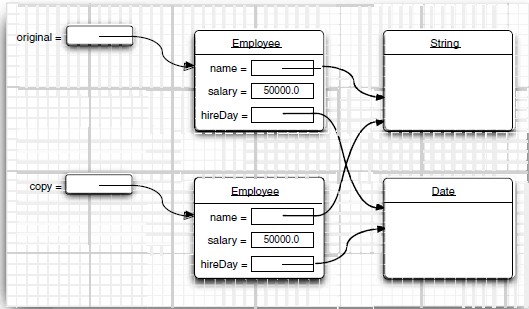
\includegraphics[scale=0.8]{images/shallow}
\caption{Shallow copy vs Deep copy\label{fig:UC3}}
\end{figure}

\subsection{Clone() con copia profonda}
\begin{figure}[H]
\centering
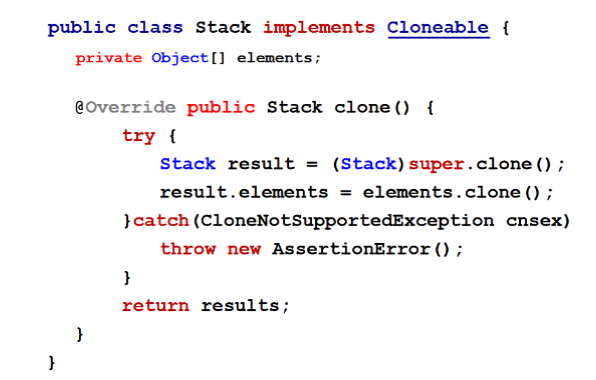
\includegraphics[scale=0.8]{images/deepCopyClone}
\caption{Deep copy Clone()\label{fig:UC3}}
\end{figure}
\begin{enumerate}
\item chiamare il metodo clone della superclasse;
\item castare il risultato al tipo stesso della classe;
\item si fa una copia profonda dei campiche hanno delle reference mutabili. Notare che su elements è stato chiamato clone()perché è il metodo che fa una copia profonda di un array di Objectma volendo si sarebbe potuto fare manualmente un for e fare deep copy del contenuto dell’array.;
\item i ritorna il risultato.
\end{enumerate}
La \textit{clone()} comunque potrebbe essere un problema se un campo è final, in generale è meglio avere un metodo di cloning separato e non implementare Cloneable.Ad esempio, si può usare un costruttore di copia oppure un factory method, ovvero un metodo che costruisce per me l’oggetto. Esempio di factory:
\begin{lstlisting}
public static Stack factoryNew(Stack source) {
Stack dest = new Stack(...);
	//faccio copie deep o altro prendendo i dati da source 
	return dest;
}
\end{lstlisting}
L’idea del factory è: creo un metodo da usare tipo Stack copia = Stack.factoryNew(...)che ritorna un oggetto di tipo Stack che è una copia esatta dell’oggetto che passoin input.
\section{La keyword \textit{final}}
La keyword \textit{final} si può utilizzare in contesti diversi ma in generale identifica qualcosa di costante o immutabile.
Il reference this, che in un metodo non statico si riferisce all'oggetto di invocazione è sempre implicitamente \textit{final}, ovvero non modificabile. Invece l'oggetto a cui this si riferisce è modificabile:
\begin{lstlisting}
public class C {
	public int x;
	public void metodo(){
		this = new C(); /* ILLEGALE: cannot assign a 
		value to final variable this*/
		this.x = 10; //ok
	}
}
\end{lstlisting}

\subsection{Campi dati final}
Un campo dati statico o no marcato \textit{final} è un campo costante / immutabile, quindi ad ogni tentativo di modifica il compilatore segna un errore.
I campi dati marcati final devono essere sempre marcati esplicitamente, non basta l'inizializzazione automatica:
\begin{lstlisting}
public class E {
final int i; // ILLEGALE
}
public class E {
static final int k; // ILLEGALE
static final int v=0; //ok
}
public class E {
final int i;
E(){i=0;} // ok
}
public class E {
final int i;
E(){i=0; i=2;} /* ILLEGALE, non posso modificare
il valore di i dopo avergli assegnato 0*/
}
\end{lstlisting}
Se un riferimento \textit{ref} viene marcato \textit{final}, allora ref si riferisce ad uno ed un solo oggetto fissato, ma il contenuto dell'oggetto puntato può essere modificato. Java non fornisce un modo per rendere costanti gli oggetti:
\begin{lstlisting}
class Z{
	int i=2;
}

public class D{
	Z z1 = new Z();
	final Z z2 = new Z();
	static final Z z3 = new Z();
	final int[] a = {1, 2, 3, 4, 5};

	public static void main(String[] args){
	D d1 = new D();
	d1.z2.i++; //ok
	d1.z1 = new Z();
	for(int i = 0; i < d1.a.lenght; i++){
	d1.a[i]++; /* ok, solamente il reference a è costante
	d1.z2 = new Z(); ILLEGALE, z2 è final
	D.z3 = new Z(); ILLEGALE, z3 è final
	d1.a = new int[3]; ILLEGALE, a è final
	}
  } 
}
\end{lstlisting}

\subsection{Metodi \textit{final}}
Un metodo marcato come \textit{final} indica che tale metodo non può essere ridefinito in eventuali sottoclassi.
I motivi per marcare un metodo final sono:
\begin{itemize}
	\item \textbf{Sicurezza}: si può pensare che un metodo \textit{boolean validatePassword()} può essere marcato final per evitare evenutali ridefinizioni maliziose;
	\item \textbf{Efficienza};
	\item \textbf{Progettuali}: a volte si desidera mettere un blocco sul metodo per evitare che una sottoclasse cambi comportamento.
\end{itemize}

\begin{lstlisting}
public class Classe{
    //attributi
    public final void MetodoNonRidefinibile(){
        //codice del metodo non ridefinibile
    }
    //codice
}
\end{lstlisting}

\subsection{Classi \textit{final}}
Marcare una classe C come final significa che non possono essere definiti sottoclassi di C. Naturalmente, tutti i metodi di una classe final sono implicitamente final, mentre i campi dati possono o meno essere marcati final.
Si noti che marcare una classe final si opera una notevole restrizione a suo utilizzo in quanto non sarebbe permesso l'estendibilità di quella classe.
\section{Classe immutabile}
Una classe è \textit{immutabile} se lo stato di un oggetto di quella classe (detto anche oggetto immutabile) non può essere modificato dopo che è stato creato.
Per esempio \textit{String} è una classe immutabile e una volta istanziata con il suo valore non cambia più.

Prima infatti abbiamo visto che la concatenazione col += di stringhe non è molto efficiente perché le stringhe, essendo immutabili,non si possono modificare e quindi il += crea una nuova stringa ogni volta.

Una classe immutabile generalmente si crea se non ha alcun membro esposto e non ha alcun setter; diciamo che è in “read only mode” e quindi in quanto tale è anche thread safe. Più avanti vedremo che i problemi avvengono quando più processi vogliono simultaneamente scrivere su una risorsa condivisa ma se tale risorsa è di sola lettura, ognuno può leggere quando vuole e quanto vuole. 

\begin{lstlisting}
public final class Immutable {
    private final int value;
    public Immutable(int value) {
        this.value = value;
    }
    public int getValue() {
        return value;
    }
}
\end{lstlisting}

\subsection{Regole per creare una classe immutabile}
\begin{enumerate}
	\item Non fornire alcun \textit{mutatore} tipo setter;
	\item Rendere la classe \textit{final} o comunque impedire l’estensione al di fuori del package di appartenenza;
	\item Rendere tutti i campi dati e i metodi \textit{final};
	\item Mettere tutti i campi dati \textit{privati};
	\item Ogni variabile membro che fa riferimento a oggetti mutabili (come ad esempio array, collezioni o la classe java.util.Date):
		\begin{itemize}
			\item va resa privata;
			\item non deve mai essere restituita all’esterno se non attraverso una sua copia;
			\item deve avere reference solo all’interno della classe; quindi nel caso in cui la variabile membro sia inizializzata nel costruttore con un oggetto mutabile, va memorizza una copia dell’oggetto al posto dell’oggetto originale;
			\item non deve essere variata dopo la costruzione dell’oggetto.
		\end{itemize}
\end{enumerate}

\subsection{Esempio pratico}
Esempio di classe mutabile:
\begin{lstlisting}
package it.cosenonjaviste.classiimmutabili.mutabile;
 
import java.text.DecimalFormat;
import java.util.EnumSet;
import java.util.Set;
 
public class Pizza {
 
  public enum Formato {
    NORMALE, BABY, MAXI, CALZONE;
  }
 
  public enum Ingrediente {
    PROSCIUTTO, FUNGHI, PATATE, SALSICCIA, CARCIOFI, SPECK;
  }
 
  protected Formato formato;
  protected Set ingredienti = EnumSet.noneOf(Ingrediente.class);
 
  public Formato getFormato() {
    return formato;
  }
 
  public void setFormato(Formato formato) {
    this.formato = formato;
  }
 
  public void aggiungiIngrediente(Ingrediente i) {
    ingredienti.add(i);
  }
 
  public void rimuoviIngrediente(Ingrediente i) {
    ingredienti.add(i);
  }
 
  public Set getIngredienti() {
    return ingredienti;
  }
 
  public double getPrezzo() {
    double prezzo = 0.0;
    switch (formato) {
    case BABY:
      prezzo += 2.0;
      break;
    case NORMALE:
    case CALZONE:
      prezzo += 4.0;
      break;
    case MAXI:
      prezzo += 7.0;
      break;
    }
    prezzo += ingredienti.size() * 1.0;
    return prezzo;
  }
 
  public String toString() {
    return formato + " " + ingredienti + " " + 
    new DecimalFormat("#,##").format(getPrezzo());
  }
 
}

/*nel main*/
Pizza prosciutto = new Pizza();
Pizzeria.pizze.add(prosciutto);
prosciutto.setFormato(Formato.CALZONE);
prosciutto.aggiungiIngrediente(Ingrediente.PROSCIUTTO);
System.out.println("Ho segnato l'ordine di " + prosciutto);
\end{lstlisting}
La stessa classe in versione immutabile:
\begin{lstlisting}
public final class Pizza {
 
  public static final Pizza MARGHERITA = 
  	new Pizza(Formato.NORMALE, EnumSet.noneOf(Ingrediente.class));
  public static final Pizza PROSCIUTTO = 
  	new Pizza(Formato.NORMALE, EnumSet.of(Ingrediente.PROSCIUTTO));
  public static final Pizza CALZONE_PROSCIUTTO = 
  	new Pizza(Formato.CALZONE, EnumSet.of(Ingrediente.PROSCIUTTO));
 
  public enum Formato {
    NORMALE, BABY, MAXI, CALZONE
  }
 
  public enum Ingrediente {
    PROSCIUTTO, FUNGHI, PATATE, SALSICCIA, CARCIOFI, SPECK
  }
 
  private final Formato formato;
  private final Set<Ingrediente> ingredienti;
  private Double prezzo;
  private String toString;
 
  public Formato getFormato() {
    return formato;
  }
 
  public Set<Ingrediente> getIngredienti() {
    return EnumSet.copyOf(ingredienti);
  }
 
  public Pizza(Formato formato, Set<Ingrediente> ingredienti) {
    this.formato = formato;
    this.ingredienti = EnumSet.copyOf(ingredienti);
  }
 
  public double getPrezzo() {
    if (prezzo == null) {
      prezzo = 0.0;
      switch (formato) {
      case BABY:
        prezzo += 2.0;
        break;
      case NORMALE:
      case CALZONE:
        prezzo += 4.0;
        break;
      case MAXI:
        prezzo += 7.0;
        break;
      }
      prezzo += ingredienti.size() * 1.0;
    }
    return prezzo;
  }
 
  public String toString() {
    if (toString == null) {
      toString = formato + " " + ingredienti + " " +
       new DecimalFormat("#,##").format(getPrezzo());
    }
    return toString;
  }
\end{lstlisting}

Esempio sbagliato:
\begin{lstlisting}
public class MyDateTime{
	private Date dateTime;
	private TimeZome tz;

	public MyDateTime(Date dateTime, TimeZone tz){
		this.dateTime = dateTime;
		this.tz = tz;
	}

	public Date getDateTime() {return dateTime;}
}
\end{lstlisting}
Non va bene qua perché sto inizializzando due classi (dateTime e tz) semplicemente facendo una copia di reference; non sto facendo una copia profonda ma sto solo copiando il puntatore. Inoltre sto ritornando una reference ad un campo oggetto privato della classe! In realtà, già solo con il costruttore sono in pericolo perché mi basta modificare l’oggetto da fuori la classe per modificarlo anche dentro dato che non ho fatto una copia profonda.
\subsection{Vantaggi}
\begin{itemize}
	\item Nessun thread può corrompere lo stato interno di una classe immutabile;
	\item  Le classi immutabili siano più semplici da programmare poiché le loro istanze possono assumere uno e un solo stato che viene mantenuto dalla costruzione in poi. 
\end{itemize}

\subsection{Svantaggi}
\begin{itemize}
	\item Dato che un oggetto immutabile non può essere variato, se si vuole effettuare una modifica sarà necessario costruire un nuovo oggetto che differisce dal primo solo per la variazione voluta;
\end{itemize}

\subsection{Differenza tra classe immutabile e oggetto immutabile}
Una \textbf{classe immutabile} genera oggetti immutabili per definizione, mentre un \textbf{oggetto immutabile} non necessariamente è instanziato da una classe anch’essa immutabile.
Esempi di oggetti immutabili:
\begin{lstlisting}
public final class Immutable2 {
    
        private final String text;
    
        public Immutable2(String text) {
            this.text = text;
        }
    
        public String getText() {
            return this.text;
        }
    }	
\end{lstlisting}

\begin{lstlisting}
public final class Immutable3 {
    
        private final String text;
    
        private Immutable3(String text) {
            this.text = text;
        }
    
        public String getText() {
            return this.text;
        }
    
        public static Immutable3 create(String text) {
            return new Immutable3(text);
        }
    }	
\end{lstlisting}

\subsection{Regole per creare oggetti immutabili}
\begin{enumerate}
	\item Tutte le proprietà devono essere settabili nel costrutture o in un metodo statico di init (vedi create sopra);
	\item Nessun setter, se necessari per qualche motivo dovrebbero sollevare un eccezione;
	\item tutte le proprietà devono essere marcate private e final;
	\item La classe deve essere marcata final;
	\item Caso in cui si riferenzi oggetti mutabili: usare deep copy per passare i valori al costruttore e per leggerli attraverso metodi di getter.
	\end{enumerate}

\subsection{Perchè la classe \textit{String} è immutabile}
\begin{itemize}
	\item \textbf{Sicurezza}: i parametri sono in genere rappresentati come String nelle connessioni di rete, url di connessione al database, nomi utente / password ecc. Se fosse mutabile, questi parametri potrebbero essere facilmente modificati;
	\item \textbf{Sincronizzazione e concorrenza}: rendere String immutable li rende automaticamente thread-safe, risolvendo così i problemi di sincronizzazione;
	\item \textbf{Caching}: quando il compilatore ottimizza gli oggetti String, vede che se due oggetti hanno lo stesso valore (a = "test" e b = "test") e quindi è necessario un solo oggetto stringa (per entrambi aeb, questi due punti allo stesso oggetto);
	\item \textbf{Caricamento della classe}: String viene utilizzato come argomento per il caricamento della classe. Se mutabile, potrebbe causare il caricamento di una classe errata (perché gli oggetti mutabili cambiano il loro stato);
	\end{itemize}
\section{Ereditarietà e composizione}

Generalmentesi tende a favorire la composizione in favore dell’eredirarietà.L’ereditarierà e l’override di metodi può essere pericoloso e più difficile di quanto ci si aspetti, proprio come accade per il metodo equals. La cosiddetta tecnica di composizione ci può salvare da questi pericoli:

\begin{lstlisting}
/*ereditarietà*/
public class Test extends Another{
	//codice...
}

/*composizione*/
public class Test {
	private Another a = ... ;
	//codice...
}
\end{lstlisting}
In pratica al posto di ereditare e fare override di metodi si usa un campo privato interno alla classe e si usa quell’oggetto all’interno di alcuni metodi che andranno definiti nella classe contenitore, in questo caso la Test.Vediamo un esempiodove si crea una classe che ne estende un’altra e ha lo scopo di contare quanti elementi sono stati inseriti.

\begin{figure}[H]
\centering
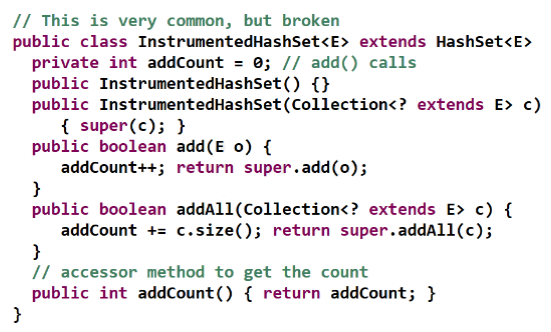
\includegraphics[scale=0.8]{images/composizione}
\caption{Ereditarietà esempio errato\label{fig:UC3}}
\end{figure}
Internamente la classe HashSet implementa addAll()basandosi su add(); in altre parole, la classe HashSet dentro al metodo addAll()chiama add(). Facendo così il metodo addCount() ritorna un numero sbagliato.
\begin{itemize}
	\item La chiamata addAll() incrementa correttamente la variabile addCount ma poi fa una chiamata a super.addAll(c);questo chiama il metodo add()che oltre a chiamare (giustamente) super.add(c);chiama anche addCount++! Quindi il conteggio totale viene sballato perché incremento addCountdi c.size()e poi anche di 1 col ++ ma non dovrei.
	\end{itemize}
	Vediamo dunque che in questo caso possiamo “favor compisition over inheritance” per risolvere il tutto:

	\begin{figure}[H]
\centering
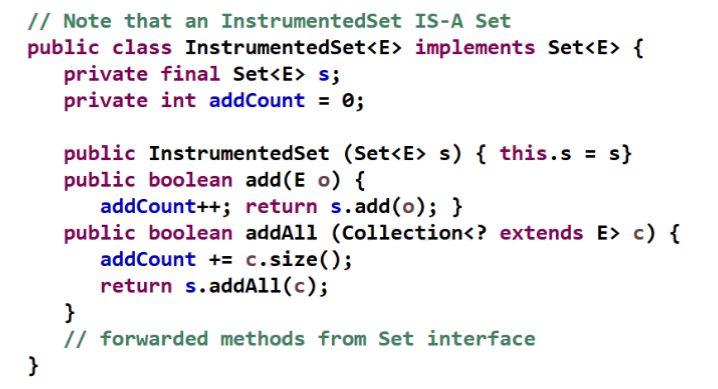
\includegraphics[scale=0.8]{images/composizione2}
\caption{Composizione esempio giusto\label{fig:UC3}}
\end{figure}
Adesso il problema non c’è più perché, avendo un oggetto interno, posso usare questo e non ho bisogno di fare override o fare chiamate a super. Implemento solamente l’interfaccia e faccio override dei contratti dei metodi specificati da quell’interfaccia (Set<E>).
\section{La keyword \textit{abstract}}
\subsection{Metodi astratti}
È possibile definire dei metodi astratti all'interno delle classi astratte. Tali metodi, dovranno essere necessariamente ridefiniti (tramite override) nelle classi figlie. 

Un metodo astratto non può essere invocato in quanto non è definito, ma potrà essere soggetto a riscrittura( override ) in una sottoclasse.
\begin{lstlisting}
public abstract void Metodo();
\end{lstlisting}
\subsection{Le classi astratte}
In java una classe può essere dichiarata astratta usando il modificatore \textit{abstract}. 

Una classe astratta è una classe \textit{incompleta}, perchè contiene dei metodi astratti, cioè metodi d'istanza senza una corrispondente implementazione.

Data una astratta \textit{AbstractC} non posso creare istanze di quella classe tramite \textit{new AbstractC()}, perchè il loro comportamento non sarebbe determinato nel caso si invocasse su di esse un metodo astratto.
\begin{lstlisting}
public abstract class A {
double campoDati1;
/*una classe che contiene almeno un metodo astratto
dev'essere marcata abstract*/
	public abstract void metodo(); 
}
\end{lstlisting}
Una classe astratta può dichiarare dei campi (che ne descrivono lo stato) e dei metodi (non astratti) che ne specificano il funzionamento, oppure delle interfacce.

\textbf{Lo scopo} e l’utilità delle classi astratte è di gestire il comportamento di base delle classi che la derivano e che può essere ampliato e specializzato da queste ultime.
E' possibile avere dei costruttori astratti soprattutto quando ci sono dei campi dati nella classe,

Una \textit{classe concreta} che estende una classe astratta deve necessariamente implementare tutti i metodi astratti della superclasse, altrimenti il compilatore segnalerà un errore.

Se una classe concreta estende una classe abstract e in più è marcata abstract, allora tale sottoclasse è considerata una classe astratta.
Esempio:
\begin{lstlisting}
public abstract class A {
	private int a;
	public A(int x) {a=x;}
	public abstract int m(); 
	}

public class C extends A { // C e' una concretizzazione di A
	private int b;
	public int m() {return 4;} // implementazione di m()
	public C() {super(8); b=0;} // OK//
	public C(int x){}// ILLEGALE: No constructor matching A() 
	//found in class A
	public static void main(String args[]) { 
	 // A r = new A(9); //ILLEGALE: Abstract class A can't be 
	 //instantiated
	 A s = new C(); // OK
	 }  
	}
\end{lstlisting}

\subsection{Cose permesse vs cose non permesse}
\textbf{Non permesso}:
\begin{itemize}
	\item Non è possibile avere metodi statici astratti, altrimenti potrebbero essere invocati tramite il nome della classe senza istanziare un oggetto di quella classe astratta;
	\item Non è possibile avere un metodo finalastratto: sarebbe un \textit{no sense};
	\item Non si possono creare oggetti di classi astratte;
\end{itemize}

\textbf{Permesso}:
\begin{itemize}
	\item E’ possibile dichiarare un reference il cui tipo (statico) è una classe astratta A: il tipo dinamico di un tale reference dovrà quindi essere una sottoclasse concreta di A. Quindi una classe astratta può essere solamente un tipo statico, mai un tipo dinamico;
	\item E` possibile definire una classe astratta ma senza alcun metodo astratto. E’ anche possibile marcare astratta una classe che non definisce dei metodi (solo stato);
	\item In una classe astratta ci possono essere dei metodi implementati che invocano metodi astratti: a run-time verrà sempre invocato virtualmente l'opportuno metodo concreto
\end{itemize}




\end{document}
